\documentclass[a4paper,onecolumn]{extarticle}
%\usepackage[left=25mm, right=25mm]{geometry}
\usepackage{geometry}
\usepackage[page,toc,titletoc,title]{appendix}
\usepackage{url}
\usepackage{caption}
\usepackage{subcaption}
\usepackage[sc]{mathpazo} % Use the Palatino font
\usepackage[T1]{fontenc} % Use 8-bit encoding that has 256 glyphs
\usepackage[utf8]{inputenc} % Use utf-8 as encoding
\linespread{1.05} % Line spacing - Palatino needs more space between lines
\usepackage{microtype} % Slightly tweak font spacing for aesthetics
\usepackage[spanish, activeacute]{babel}
 \decimalpoint
% \usepackage[hmarginratio=1:1,top=32mm,columnsep=20pt]{geometry} % Document marginshttps://www.overleaf.com/project/60211b96f72a79d4c7515e93
% \usepackage[hang, small,labelfont=bf,up,textfont=it,up]{caption} % Custom captions under/above floats in tables or figures
\usepackage{verbatim} % comentarios
\usepackage{listings}
\usepackage{xcolor}
\usepackage{wrapfig}
\lstset{
    inputencoding=utf8,
    frame=single,
    basicstyle=\fontsize{7}{10}\selectfont\ttfamily,
    basicstyle=\ttfamily\small,
    keywordstyle=\color{blue}\bfseries,
    identifierstyle=\color{black},
    commentstyle=\color{gray}\itshape,
    stringstyle=\color{red},
    numbers=left,
    numberstyle=\tiny\color{gray},
    stepnumber=1,
    numbersep=10pt,
    showspaces=false,
    showstringspaces=false,
    breaklines=true,
    breakindent=0pt,
    breakatwhitespace=false,
    tabsize=2,
    captionpos=b,
    literate={á}{{\'a}}1
        {ã}{{\~a}}1
        {é}{{\'e}}1
        {ó}{{\'o}}1
        {í}{{\'i}}1
        {ñ}{{\~n}}1
        {¡}{{!`}}1
        {¿}{{?`}}1
        {ú}{{\'u}}1
        {Í}{{\'I}}1
        {Ó}{{\'O}}1
}
\setlength{\parskip}{0.8em}
\usepackage{natbib}
\usepackage{enumitem}
% \setlist[itemize]{noitemsep} % Make itemize lists more compact
% \usepackage{abstract} % Allows abstract customization
% \renewcommand{\abstractnamefont}{\normalfont\bfseries} % Set the "Abstract" text to bold
% \renewcommand{\abstracttextfont}{\normalfont\small\itshape} % Set the abstract itself to small italic text
\usepackage{titlesec}

\usepackage{fancyhdr} % Headers and footers
\pagestyle{fancy} % All pages have headers and footers
\fancyhead{}
\fancyhead[LE,RO]{Hugo Gómez Sabucedo}
\fancyhead[RE,LO]{Aplicación de ML para predicción de rendimiento de acciones}

\renewcommand{\footrulewidth}{0.2pt}
\usepackage{titling} % Customizing the title section
\usepackage[breaklinks=true]{hyperref} % For hyperlinks in the PDF
%\usepackage{array}
%\newcolumntype{C}[1]{>{\centering\let\newline\\\arraybackslash\hspace{0pt}}m{#1}}
\usepackage{graphicx}
%\usepackage{lipsum} % NO NECESARIO LUEGO
%\usepackage{amsmath}
%\usepackage{wrapfig}
%\usepackage{multicol}
%\usepackage{bm}


\let\stdsection\section
\renewcommand\section{\newpage\stdsection}

%-------------------------------------------------------------------------------
%	TITLE SECTION
%-------------------------------------------------------------------------------

\setlength{\droptitle}{-4\baselineskip} % Move the title up



\title{\begin{center} \Huge Trabajo Final de Máster: \\ Aplicación de algoritmos de Machine Learning para predicción de rendimiento de acciones\end{center}} % Article title
\author{
    \textsc{\huge Hugo Gómez Sabucedo} \\ % Your name
    \large \href{mailto:hugogomezsabucedo@gmail.com}{hugogomezsabucedo@gmail.com} \\ [2ex] % Your email address
    \Large \textbf{Máster Big Data, Data Science \& Inteligencia Artificial} \\
    \normalsize Curso 2024-2025 \\
    \large Universidad Complutense de Madrid
}
\date{} % Leave empty to omit a date

\begin{document}
% Print the title
\maketitle
\setcounter{tocdepth}{4}
\tableofcontents
\listoffigures
%\listoftables
\begin{sloppypar}

%-------------------------------------------------------------------------
%	DOCUMENT
%-------------------------------------------------------------------------

\section{Introducción al problema} \label{introduccion}
\renewcommand\section{\stdsection}
\subsection{Introducción y objetivos} \label{intro}
El análisis de datos e información financiera es una tarea altamente compleja ya que, al contrario de lo que ocurre en otras series temporales (por ejemplo, 
de datos de turismo o de viajes), no tienden a ser tan regulares, oscilando mucho ya no sólo de un día a otro, sino en una misma jornada. Además, a la hora
de invertir, se busca obtener no sólo el máximo rendimiento en términos absolutos, sino de forma proporcional: es decir, ganar lo máximo posible, invirtiendo 
no mucho dinero. Es importante también tener en cuenta el posible riesgo de la inversión, así como el entorno que rodea a la misma: si invertimos en una empresa
que viene creciendo a un ritmo vertiginoso, es posible que rápidamente deje de crecer o se estanque, con lo que el rendimiento obtenido no sería tan alto como el
esperado. Por otra parte, invertir en una empresa que viene reduciendo su cotización no siempre puede ser una buena idea: si esta reducción se produce en un contexto 
global, podría ser una buena inversión, ya que lo más probable es que vuelva a crecer y se gane dinero; pero si esto se produce en un contexto local, lo más probable 
es que esa empresa no se recupere, o no lo haga tan rápidamente.

Es por ello que, para poder realizar estas preidcciones, se propone este Trabajo de Final de Master, en el que se analizará un dataset disponible en Kaggle que contiene 
información financiera de las 500 empresas del índice bursátil SP\&500 de Estados Unidos. Por tanto, el objetivo de este trabajo será, empleando estos datos, crear y
comparar distintos modelos y técnicas de Machine Learning, encontrando el mejor de ellos para predecir el rendimiento de las acciones y poder decidir en qué empresa
se debería invertir para obtener un mayor rendimiento.

Para ello, en primer lugar, se realizará una análisis descriptivo de los datos, y se transformarán y limpiarán para asegurar que tienen el formato correcto. Una vez 
tenemos el dataset adecuado, se crearán los distintos modelos (en este caso, se ha optado por combinar un XGBoost, LightGBM, LSTM, GRU y Conv1D) para entrenarlos sobre 
una submuestra de los datos, y se compararán las métricas de los mismos, para definir cuáles son los mejores. Sobre estos tres mejores, se aplicará un bagging, con el
objetivo de reducir la varianza de los modelos y obtener uno más robusto. Una vez obtenido el modelo final, se reentrenará con los datos de todas las empresas,
para poder finalmente realizar las predicciones.

\section{Análisis descriptivo y transformaciones} \label{analisis_transformaciones}
El primer paso es, naturalmente, cargar los datos y realizar un análisis preliminar de los mismos. El código completo de este análisis se encuentra en el anexo 
\ref{Anexo:EDA}. En este análisis preliminar, en la figura \ref{fig:EDAPreliminar} podemos ver que la serie contiene datos para un total de 491 empresas desde el 29 de noviembre de 2018 hasta el 29 de
noviembre de 2023; es decir, un total de 5 años exactos. Si analizamos las empresas en función del número de datos que tienen vemos que en el top 10 de empresas con 
más registros todas tienen el mismo número, 1258, una cifra cercana a lo esperado (teniendo en cuenta que, si en estos cinco años de datos excluimos los fines de 
semana, días en las que los mercados financieros no abren, tendríamos un total de 1300 días, a los que habría que restar posibles festivos, etc.). Sin embargo, en el
top 10 de empresas con menos datos, hay numerosas empresas con la mitad o más de sus datos faltantes. Posteriormente se explicará como se tratarán estos casos.
\begin{figure}[h]
    \centering
    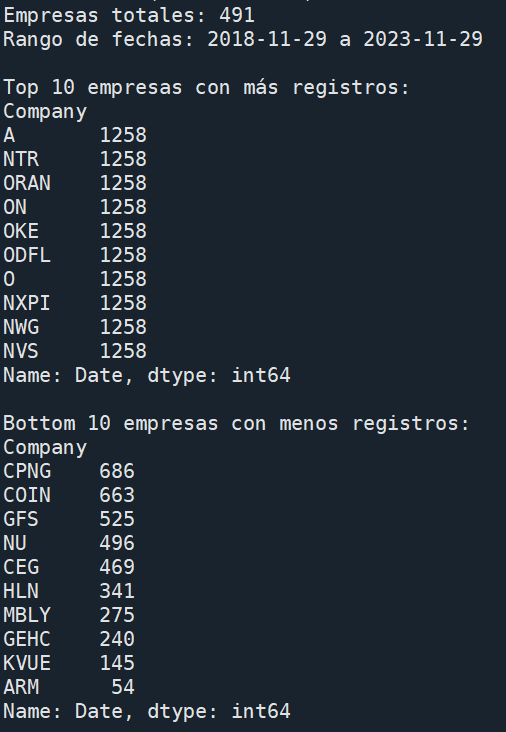
\includegraphics[width=0.25\textwidth]{imgs/EDA/eda_preliminar.png}
    \caption{EDA preliminar} \label{fig:EDAPreliminar}
\end{figure}

Visto que el dataframe carece de datos para los fines de semana, lo cual dejaría puntos en la serie temporal sin datos, se ha decidido hacer un resampleo de los 
mismos con una frecuencia semanal, calculando la media de los datos de esa semana. De esta forma, nos aseguramos de tener una serie de datos consistentes con la
que trabajar. Este resampleo, sin embargo, presenta una desventaja, ya que perderemos cierta granularidad en los datos y la posibilidad de registrar mejor ciertas
subidas o bajadas bruscas que se produzan de un día para otro. Pero, por otra parte, como se ha comentado, se gana en consistencia en los datos y también en eficiencia
computacional, ya que tenemos que tener en cuenta que el conjunto inicial de datos con el que trabajamos tiene alrededor de 603,000 filas. Además, se ha pivotado el dataframe,
de forma que trabajemos con un conjunto de datos cuyo índice sea la fecha (en este caso, semana); las columnas, las distintas empresas; y vayamos almacenando los valores. 

\begin{figure}[h!]
    \centering
    \begin{subfigure}{0.2\textwidth}
        \centering
        
\includegraphics[width=\textwidth]{imgs/eda/missing_empresa.png}
        \caption{Valores missing por empresa} \label{fig:missingCompany}
    \end{subfigure}
    \hfill
    \begin{subfigure}{0.75\textwidth}
        \centering
        
\includegraphics[width=\textwidth]{imgs/eda/missing_date_pre.png}
        \caption{Valores missing por fecha} \label{fig:missingDatePre}
    \end{subfigure}
    \caption{Valores missing}
\end{figure}


Con estos pasos, se ha reducido el dataset a uno de 262 filas por 491 columnas. El siguiente paso será analizar el porcentaje de valores missing por empresa y por fecha, como se ve 
en las figuras \ref{fig:missingCompany} y \ref{fig:missingDatePre}. En este caso, observamos que el top 10 de empresas con más valores faltantes tiene un porcentaje de más del 40\%,
y vemos que, según nos acercamos al presente, el número de missing por fecha va reduciéndose. Esto nos indica que son empresas que se crearon posteriormente a la fecha de inicio 
de los datos, o que empezaron a cotizar en bolsa después de esta fecha. Por tanto, para tratar los valores missing, se usarán dos estrategias.
\begin{itemize}
    \item En primer lugar, se ha definido un umbral máximo sobre el porcentaje de valores missing que puede tener una empresa, que en este caso se ha establecido como un 40\%, 
    y se eliminarán por completo estas empresas. Esto se debe a que se considera que será complejo interpolar los datos para rellenar con los valores faltantes y que, además, 
    no tendría mucho sentido. Como se ha visto, son empresas que han empezado a cotizar en bolsa en años intermedios del dataset, por lo que, si para más de la mitad de los años 
    que analizamos no tenemos sus datos, no tiene mucho sentido incluirlas al análisis. Las empresas que se eliminarán se pueden ver en la figura \ref{fig:NANpercent}.
    \item La otra estrategia, para las empresas que presenten menos de un 40\% de valores faltantes, se realizará una interpolación de los mismos. En este caso, indicando el índice 
    como un eje temporal, se realiza una interpolación con \texttt{bfill} o \textit{backward fill}. Es decir, se rellenan los valores missing con el siguiente valor válido hacia
    atrás, de forma que se usa el primer valor válido que haya después de los NaN para rellenarlos con ese valor.
\end{itemize}

\begin{figure}
    \centering
    
\includegraphics[width=\textwidth]{imgs/eda/na_by_percent.png}
    \caption{Empresas con NaN $>= 40\%$} \label{fig:NANpercent}
\end{figure}

Se han elegido estas estrategias, especialmente la de la interpolación temporal con bfill, ya que se han considerado las más adecuadas. Evidentemente, una interpolación con un valor fijo
no tendría sentido, ya que distorsiona la serie, al igual que rellenar con medidas estadísticas como la mediana o la moda. Una interpolación polinómica podría no ser tampoco 
la más adecuada, ya que en series con mucha variabilidad o datos atípicos no funciona adecuadamente. Es por ello que se ha elegido la interpolación temporal, ya que mantiene la coherencia 
temporal de los datos, algo crucial. De esta forma, tras la aplicación de estas técnicas, tenemos unos datos perfectamente limpios.

\begin{figure}
    \centering
    
\includegraphics[width=0.6\textwidth]{imgs/eda/descr_top10.png}
    \caption{Análisis descriptivo de las 10 primeras empresas} \label{fig:Descriptivos10}
\end{figure}

El siguiente paso es realizar un muy breve análisis descriptivo de los datos, en este caso para las 10 primeras empresas. Se puede observar una variabilidad en los precios, 
con empresas como AAPL (Apple) con desviaciones estándar elevadas teniendo en cuenta las medias. En general, las medias y medianas (50\%) son cercanas, lo que indica que, 
pese a las fluctuaciones, estas no son excesivamente elevadas. De todas formas, estos datos nos podrían indicar una ligera volatilidad, lo cual se debe tener en cuenta en los análisis futuros,

\begin{figure}
    \centering
    
\includegraphics[width=0.75\textwidth]{imgs/eda/top20_seasonal.png}
    \caption{Empresas según su fuerza estacional} \label{fig:fuerzaEstacional}
\end{figure}

A continuación, se analiza la fuerza estacional de las series, para ver qué empresas presentan una mayor fuerza estacional. Para ello, se hace la descomposición estacional de la serie,
teniendo en cuenta que trabajamos con series temporales anuales (un periodo de 52 semanas), y calculamos la fuerza estacional, que es la relación entre la varianza del componente 
estacional de la serie y la varianza total de la serie. Así, se obtiene el gráfico de la figura \ref{fig:fuerzaEstacional}, donde se ven las 20 empresas con mayor fuerza estacional. 
Esta clasificación la emplearemos para calcular la descomposición de la serie en sus componentes, como se ve en la figura \ref{fig:descomposiciones}.

\begin{figure}[h!]
    \centering
    \begin{minipage}{0.49\textwidth}
        \centering
        
\includegraphics[width=\textwidth]{imgs/eda/descomposicion_max_PPL.png}
        \caption{Descomposición estacional de PPL} \label{fig:descMax}
    \end{minipage}\hfill
    \begin{minipage}{0.49\textwidth}
        \centering
        
\includegraphics[width=\textwidth]{imgs/eda/descomposicion_med_SHEL.png}
        \caption{Descomposición estacional de SHEL} \label{fig:descMed}
    \end{minipage}\\[1ex]  

    \begin{minipage}{0.49\textwidth}
        \centering
        
\includegraphics[width=\textwidth]{imgs/eda/descomposicion_min_MCK.png}
        \caption{Descomposición estacional de MCK} \label{fig:descMin}
    \end{minipage}\hfill
    \begin{minipage}{0.49\textwidth}
        \centering
        
\includegraphics[width=\textwidth]{imgs/eda/series_comparacion.png}
        \caption{Comparación de las series} \label{fig:seriesPlot}
    \end{minipage}
    \caption{Descomposiciones estacionales} \label{fig:descomposiciones}
\end{figure}

Se ha elegido la serie con mayor fuerza estacional (PPL, figura \ref{fig:descMax}), con menor fuerza estacional (MCK, figura \ref{fig:descMin}) y la mediana (SHEL, figura 
\ref{fig:descMed}). Además, en la figura \ref{fig:descomposiciones}, podemos ver las tres series dibujadas juntas (aunque cada serie individual se puede ver también en su
figura respectiva). La descomposición temporal de las series nos da cuatro gráficos distintos:
\begin{enumerate}
    \item El \textbf{componente observado}, que es la serie temporal tal y como es, con todos sus valores.
    \item El \textbf{componente de tendencia}, que captura la dirección a largo plazo de la serie. En este caso, se ve una tendencia creciente en las tres empresas, pero con ligeras
    diferencias. Mientras que la primera empresa se ve una tendencia creciente, que se vio interrumpida por la pandemia, para luego sufrir de nuevo un crecimiento explosivo y un 
    estancamiento; en la segunda empresa se observa simplemente la caída debida a la pandemia y el posterior crecimiento, en una tendencia ascendiente que aún no se ha cortado; y en 
    la última empresa, se ve un crecimiento constante, menor o menos abrupto los primeros años (coincidentes también con la pandemia)
    \item El \textbf{componente estacional}, que captura los patrones o ciclos en los datos. Estos patrones pueden deberse a numerosas causas, como el clima, festividades, las estaciones, etc.
    Representa las fluctuaciones que ocurren, para el mismo período (en este caso, anual), en cada ciclo (por ejemplo, se observa que, por lo general, al inicio del año, los 
    precios sufren una bajada, precedida de una subida en los últimos meses del año). Es crucial para el análisis, ya que nos permite saber si podremos predecir estos patrones 
    correctamente.
    \item El \textbf{componente residual}, la variabilidad aleatoria que no se explica ni por la tendencia ni por la estacionalidad. Se corresponde con anomalías o eventos únicos, ruido, 
    por lo cual, como es esperable, nuestras series presentan ciertos residuos. Sin embargo, lo importante es que estos estén incorrelados, que sean aleatorios. Si aplicamos la prueba de
    Ljung-Box sobre los residuos, que evalúa precisamente si existe una autocorrelación significativa, obtenemos p-valores extremadamente pequeños, del orden de $10^{-100}$.
    En este caso, nos indicaría que los residuos no son aleatorios. Sin embargo, esto puede deberse a que esta descomposición se hace usando modelos relativamente simples, lineales, 
    y que podríamos necesitar modelos más complejos para analizar series complejas como las que tenemos.
\end{enumerate}

Por último, una vez que hemos realizado el análisis al completo y que hemos limpiado los datos, vamos a realizar una exportación del dataset ya limpio, para poder usarlo como 
base de trabajo en los sucesivos códigos y no tener que realizar la limpieza cada vez que se ejecutan.

\section{Modelos: creación y aplicación} \label{modelos}
En esta sección se comentará el bloque principal de este trabajo: los modelos. Se explicará cuáles se han elegido y el porqué, comentando sus ventajas y desventajas. Se comentará también 
como se han creado y entrenado, así como los parámetros empleados, explicando las decisiones tomadas. Se analizarán los resultados y métricas obtenidas, y se explicará el proceso de bagging 
empleado para mejorar los modelos, con sus correspondientes métricas y resultados.

\subsection{Elección de modelos} \label{eleccion}
Para este trabajo se han elegido cinco modelos principales, cada uno de los cuales aporta numerosas ventajas y desventajas. Además, se han desarrollado tres scripts distintos 
como parte de la elección no sólo del mejor modelo, sino de la forma de predecir los datos. Por una parte, tenemos en el anexo \ref{Anexo:H1} un código que entrena los modelos y 
realiza predicciones para una predicción a corto plazo, de una semana; por otra parte, en el anexo \ref{Anexo:H4}, un código que realiza el entrenamiento y predicción en un horizonte
a medio plazo de 4 semanas; y por último, en el anexo \ref{Anexo:Comb}, un framework combinado.

El motivo de haber desarrollado estos tres códigos, aunque realmente son similares entre ellos, es un enfoque progresivo del problema. Aunque en todos los casos se emplean 
los mismos modelos, la diferencia radica en el horizonte temporal de salida: mientras que en el caso de H=1 los modelos se centran en predecir un único paso, los modelos con 
H=4 deben predecir a un mes vista, cambiando el enfoque del problema a una predicción multihorizonte. Esto, pese a mantener la estructura de los modelos, incrementa la 
dificultad del aprendizaje de los mismos y suele afectar también a la precisión de las predicciones, ya que tienen el reto no sólo de predecir con mayor o menor exactitud 
el siguiente valor de la serie, sino la tendencia y evolución de la serie. Finalmente, el framework combinado se concibió como una manera de tener una mejor visión de los 
resultados de los modelos, ya que evidencia cuál de los dos casos genera mejores predicciones. De este modo, la combinación de las tres versiones enriquece también el análisis.

En lo que a los modelos respeta, se han elegido cinco tipos diferentes: XGBoost, LightGBM, LSTM, GRU y Conv1D.

\subsubsection{Modelos de árboles} \label{modelos}
Los modelos de árboles se basan en la combinación, mediante \textit{gradient boosting}, de árboles de decisión ``débiles`` secuencialmente, de forma que cada árbol nuevo 
corrige los errores del anterior. Aprenden minimizando una función de pérdida y cada iteración añade un árbol entrenado sobre los residuos. Son buenos para capturar no linearidades
e interacciones entre variables, pero no comprenden el orden temporal, por lo que les tendremos que proporcionar ventanas como features, como se explicará en \ref{preparacion}.
Dentro de este tipo se encuentran los modelos de \hyperref[XGB]{XGBoost} y \hyperref[LGBM]{LightGBM}.

En el contexto de este trabajo, son adecuados ya que, tras la creación de las ventanas temporales, los datos presentan una estructura tabular, con la que cada fila representa un 
bloque de $W$ semanas y la variable objetivo se correspode con la semana siguiente (o las cuatro siguientes). Esto es fácilmente manejable por estos algoritmos, capturando 
las relaciones no lineales entre ellos.

\paragraph{XGBoost} \label{XGB}\mbox{} \\
XGBoost, o \texttt{eXtreme Gradient Boosting}, es un algoritmo de aprendizaje supervisado que implementa una técnica llamada \textit{gradient boosting}. En esta técnica se 
entrenan secuencialmente múltiples árboles de decisión, de forma que cada nuevo árbol corrija los errores cometidos por los anteriores optimizando una función de pérdida. Su 
principal ventaja es que usa la memoria muy eficientemente y tiene una estructura optimizada para que las predicciones y las construcciones de los árboles sean fácilmente escalables.
Esta técnica, además permite controlar el sobreajuste si se controlan o modifican adecuadamente los hiperparámetros, pero presenta la desventaja de necesitar ventanas muy largas 
para ver bien el pasado y puede ser muy costoso con árboles muy profundos.

Los parámetros que se pueden configurar para estos modelos, y los que se usarán en este trabajo, son tres:
\begin{enumerate}
    \item \textbf{n\_estimators}: representa el número de árboles; a mayor número de árboles, mejores resultados, pero también hay más riesgo de \textit{overfitting}.
    \item \textbf{max\_depth}: representa la profundidad máxima de cada árbol, y premite limitar la complejidad.
    \item \textbf{learning\_rate}: representa cuánto aporta cada nuevo árbol; cuanto más pequeño es el valor, más robusto es el modelo, pero más lento de entrenar.
\end{enumerate}

\paragraph{LightGBM} \label{LGBM}\mbox{} \\
LightGBM, o \texttt{Light Gradient Boosting Machine}, es otra forma de implementación de boosting de árboles, diseñado con el objetivo de ser eficiente tanto en el tiempo 
que requieren para ser entrenados como en el uso de la memoria. Usa histogramas y crecimiento \textit{leaf-wise} que, al contrario de los modelos tradicionales (o \textit{depth-wise},
que trabajan dividiendo horizontalmente los árboles en cada nivel, generando árboles más anchos), trabaja seleccionando la hoja más prometedora (con mayor \textit{gain}) para dividir
el árbol. Esto acelera mucho la creación del árbol, pero también implica mayor riesgo de sobreajuste.

Para este modelo, se configurarán también los mismos parámetros que en en anterior.

\subsubsection{Modelos secuenciales}
Estos modelos procesan los datos en un orden temporal, manteniendo un estado oculto o memoria. Aprenden combinando, en cada paso, la entrada actual con el estado anterior, 
produciendo un nuevo estado, con compuertas controlando qué información se mantiene o se olvida. Son muuy buenas para capturar dependencias en series temporales, tanto a corto 
como a largo plazo, así como estacionalidades de las mismas. Sin embargo, son más costosos de entrenar y sensibles a escalados de los datos y a \textit{overfitting}. Son los 
modelos más complejos. Dentro de este tipo se encuentran los modelos de \hyperref[LSTM]{LSTM} y \hyperref[GRU]{GRU}.

En el contexto de este trabajo, con series con información de numerosos meses y en las que cambios repentinos en los datos son habituales, son modelos muy apropiados, ya que 
permiten tener en cuenta no sólo los datos de las semanas más inmediatamente recientes, sino también la trayectoria de la serie y su inercia. Esto presenta una ventaja importante 
sobre los modelos de árboles, permitiendo ajustar los datos con la información que tienen del largo plazo y saber si venían en una tendencia creciente o decreciente.

\paragraph{LSTM} \label{LSTM}\mbox{} \\
Las LSTM, o \texttt{Long Short-Term Memory}, son un tipo de red neuronal recurrente (RNN) que incorporan una memoria a largo plazo con el objetivo de recordar información durante 
secuencias largas. Están compuestas por células, cada una de las cuales tiene dos estados: un estado oculto, que es el que se transmite de paso en paso y se usa para generar la 
salida; y un estado de celda (o cell state), que es el que actúa como memoria a largo plazo. El flujo de la información se controla mediante tres \textit{gates}: la \textit{forget 
gate}, que decide qué parte de la memoria anterior se descarta; la \textit{input gate}, que decide qué nueva información se guarda; y la \textit{output gate}, que controla qué 
parte de la memoria influye en la salida.

Los parámetros que se ajustarán para este modelo son:
\begin{enumerate}
    \item \textbf{units}: el número de células ocultas de la red.
    \item \textbf{dropout}: una forma de regularización, que inactiva ciertas neuronas para que las restantes aprendan de forma más robusta.
\end{enumerate}

\paragraph{GRU} \label{GRU}\mbox{} \\
Las GRU, o \texttt{Gated Recurrent Unit}, son una variante simplificada de las LSTM, que mantienen tanto la idea de la memoria como de las puertas, pero fusionando algunas de ellas, 
con lo que logran reducir los parámetros y acelarar el entrenamiento. Cadaa unidad GRU tiene ahora un único estado oculto, controlado por dos puertas: la \textit{update gate}, que 
decide cuánto se mantiene del estado anterior; y la \textit{reset gate}, que decide cuánto se olvida.

En este caso, también se ajustarán los mismos parámetros que para las LSTM.

\subsubsection{Modelos convolucionales}
Estos modelos presentan una complejidad intermedia entre los modelos de árboles y los secuenciales. Su idea básica es aplicar filtros o kernels que van barriendo y analizando 
la secuencia y detectando patrones locales, bien sean tendencias u oscilaciones, en las ventanas. Aprenden usando pequeñas cuadrículas, llamadas \textit{kernels} o núcleos, que 
se van desplazando sobre los datos y generando mapas de activación. Su ventaja es que permiten combinar varias capas, cada una detectando un patrón o tendencia específica. Tienen 
la ventaja de capturar muy bien patrones locales repetitivos y de corto plazo, además de ser rápidos y fácilmente paralelizables. Dentro de este tipo de modelos se usará el \hyperref[C1D]{Conv1D}.

\paragraph{Conv1D} \label{C1D}\mbox{} \\
Las Conv1D, o \texttt{Convolutional Neural Network 1D}, son un tipo de red neuronal que, en lugar de procesar los datos paso a paso, aplican filtros deslizantes que los van recorriendo 
y detectando patrones locales. Funcionan con filtros convolucionales, que no son más que vectores de pesos que se desplazan sobre la secuencia de estado y van calculando, para cada 
posición, una combinación lineal de los valores de la ventana. Cada filtro aprende un patrón específico (que puede ser tendencias ascendentes en el último mes, por ejemplo) de forma que,
combinando el uso de varios filtros en paralelo, se aprenden numerosos patrones. Tras la convolución, se usan capas adicionales para aplanar y combinar las características.

Para este modelo se ajustarán, al igual que los anteriores, las \textbf{units} y el \textbf{dropout}, así como el \textbf{kernel\_size}, que modifica la longitud del kernel en pasos de tiempo.

\subsection{Preparación y configuración de modelos} \label{preparacion}
\subsubsection{Creación de datos supervisados} \label{supervisados}
Un aspecto crucial a tener en cuenta a la hora de comenzar a trabajar con los modelos es la necesidad de transformar los datos en un problema supervisado, lo que se 
conoce como \textit{ventanización} o \textit{windowing}. Esto es necesario porque los modelos que se entrenan requieren recibir los datos en forma de pares de entrada-salida, y la serie
de datos en crudo (una simple columna de precios a lo largo del tiempo) no lo es. De esta forma, el dataset restante tendrá la siguiente forma: $X_t = \left[ y_{t-W+1}, y_{t-W+2}, \dots, y_t \right]$

Para los modelos de árboles, ya que no entienden de orden temporal, si no se proporcionan los datos en forma de ventana sólo verían una columna de valores sin contexto. En el 
caso de las RNN, aunque pueden procesar secuencias, necesitan un tamaño fijo de entrada, con el que saber cuántos pasos para atrás mirar para hacer la predicción. Para esto, se 
ha realizado una función que, en base al tamaño de ventana definido y al horizonte de predicción, genera unos nuevos datos donde la entrada son las últimas $W$ observaciones, y la salida 
es 1 o 4 (en función de H) observaciones futuras.

Respecto a la elección del tamaño de la ventana, se ha optado por un tamaño de 25 semanas (aproximadamente 6 meses), ya que se ha considerado un tamaño equilibrado entre la captura
de suficiente contexto histórico para reflejar correctamente las tendencias a largo plazo y la reducción del ruido. Una ventana muy corta, de unas 3-5 semanas, haría que el modelo 
sólo observase fluctuaciones recientes, y que no detectase correctamente las tendencias. Una ventana muy larga, de por ejemplo 100 semanas, incluiría datos demasiado antiguos, que 
diluiría la información más reciente (crucial, para detectar tendencias inmediatas) y ralentizaría mucho el entrenamiento. Es, por tanto, un punto intermedio. Además, para 
el horizonte de predicción que se ha definido (bien sea el de una semana o el de cuatro), es un tamaño adecuado, ya que no se necesita información, por ejemplo, de dos años, para
predecir el rendimiento de la próxima semana.

\subsubsection{\textit{Tuning} de hiperparámetros y métricas} \label{hiperparametros}
Como se comentó en \ref{modelos}, cada uno de los modelos que se emplean tienen una serie de hiperparámetros que condicionan no sólo su capacidad de aprendizaje, sino cómo 
se comportan frente al sobreajuste de los datos o qué límite tienen a la hora de parar. A diferencia de los parámetros internos que tienen cada uno de ellos, que se van 
ajustando automáticamente, los hiperparámetros se deben establecer de forma externa.

Para ello, se ha aplicado una \textit{grid search}, en la que se define un espacio discreto de valores para cada uno de los posibles hiperparámetros y se entrena el modelo 
sucesivamente con cada una de las combinaciones. Este es un enfoque que, si bien es computacionalmente costoso, permite explorar una serie de valores razonables, obtenidos a 
partir de experimentos realizados tanto sobre los mismos datos como analizando los valores que se suelen usar más frecuentemente. Cabe destacar que los valores que se presentan 
en los códigos de los anexos no son todos con los que se ha probado, ya que previamente se ha hecho una búsqueda más extensa, con el objetivo de ajustarlos y eliminar aquellos 
con peores resultadoos.

Relacionado con los hiperparámetros, conviene hablar de las métricas empleadas para medir el rendimiento de los modelos. En este caso, se ha definido una función propia que computa 
a la vez distintas métricas para el mismo modelo:
\begin{itemize}
    \item \textbf{$R^2$} (Coeficiente de determinación). Es la métrica por excelencia, que mide la proporción de la varianza de la variable dependiente que es explicada por el modelo. 
    Valores próximos a 1 indican que el modelo explica perfectamente los datos, mientras que próximos a 0 indican que el modelo no mejora respecto a predecir siempre la media. Es el
    criterio que usaremos como principal a la hora de determinar el mejor modelo.
    \item \textbf{MSE} (Mean Squared Error). Se calcula como la media de los cuadrados de las diferencias entre los valores reales y los predichos, y es útil ya que penaliza 
    fuertemente los errores grandes (debido a la elevación al cuadrado), aunque no es interpretable en las mismas unidades que los datos originales
    \item \textbf{MAE} (Mean Absolute Error). Similar al anterior, pero mide únicamente la media de las diferencias absolutas. Es más robusto frente a valores atípicos o excesivamente 
    altos, e indica, en promedio, cuánto se desvía la predicción de los valores reales, con la ventaja de hacerlo en las unidades de la variable.
    \item \textbf{RMSE} (Root Mean Squared Error). Es simplemente la raíz cuadrada del MSE, lo que lo hace más interpretable al devolver el error medio, ahora sí, en las mismas unidades 
    que los datos.
    \item \textbf{MAPE} (Mean Absolute Percent Error). Mide el error relativo en porcentaje. Tiene la ventaja de ser intuitivo (por ser un porcentaje), pero no funciona bien con
    valores próximos a cero. En este caso, nos sirve para comparar empresas con diferentes escalas de precios
    \item \textbf{EVS} (Explained Variance Score). Mide cuánta varianza de los datos es explicada por el modelo, de forma similar al $R^2$, pero más centrada en la dispersión de los 
    errores.
    \item \textbf{DA} (Directional Accuracy). Se emplea en algunos casos para evaluar si el modelo predice correctamente la dirección del cambio (es decir, si el modelo acierta cuando 
    la serie sube o baja respecto al valor anterior). Es muy útil, ya que en nuestro caso seguramente sea más útil predecir bien la tendencia que el valor exacto.
\end{itemize}

\subsubsection{Validación cruzada} \label{crossval}
A la hora de evaluar los modelos, es importante comprobar que las métricas que hemos obtenido reflejen su capacidad de generalización a datos que no se le han proporcionado como 
conocimiento. En problemas de regresión o clasificación, suele ser suficiente con realizar una validación cruzada de los datos, dividiéndolos en particiones de entrenamiento y de test.
Sin embargo, en datos con una estructura temporal, como los nuestros, esta validación cruzada es inapropiada, ya que rompería la propia secuencialidad de los datos, produciendo un 
\textit{data leakage} (cuando los modelos se entrenan con información futura). 

Es por ello que, en este caso, se ha optado por emplear una validación cruzada, pero temporal (denominada \texttt{TimeSeriesSplit}). Este método genera divisiones sucesivas de los 
datos, en donde cada conjunto de entrenamiento contiene únicamente observaciones pasadas, y el conjunto de validación contiene valores futuros, que no se emplean en el entrenamiento. 
Así, combinamos el respeto por el orden cronológico y se simulan condiciones reales de predicción.

En este caso, se han empleado un número variable de particiones en función del tipo de modelo con el que se trabaja. Para modelos de árboles de decisión, debido a que presentan un 
menor coste computacional, se han utilizado cinco particiones; mientas que para los modelos secuenciales y convolucionales, de mayor complejidad, se han empleado únicamente tres 
particiones. Cada partición se evalúa con las métricas comentadas en \ref{hiperparametros}, y los resultados obtenidos se corresponden con la media de las métricas a lo largo de 
todos los \textit{folds}.

\subsubsection{Entrenamiento de los modelos} \label{training}
Este proceso es la parte central del trabajo, pues es donde se entrena a los algoritmos para que identifiquen los patrones y realicen las predicciones. Como se comentó en 
\ref{supervisados}, se emplearán estos datos transformados, tanto para los casos en el que se emplea el horizonte de 1 semana como para el de 4, ya que se ha diseñado una 
función que crea los datos teniendo en cuenta ambos parámetros. Sin embargo, estos datos no son los que se empleen directamente para entrenar los modelos, sino que primero 
deben escalarse, empleando un \texttt{StandardScaler}. Esto se hace para homogeneizar las escalas de los datos, y evitar que empresas con precios de las acciones muy elevados 
dominen los modelos y tiren de las predicciones. Además, se realiza un aplanado de los datos en vectores para los modelos de árboles, mientras que se conservan como tensores 
tridimensionales para las redes neuronales, para ser consistentes con las dimensiones de los datos que necesitan cada uno de los modelos.

Una particularidad a destacar de esta fase de entrenamiento es que el entrenamiento y ajuste inicial de los hiperparámetros se realiza inicialmente sobre un subconjunto aleatorio 
de un 40\% de las compañías. Esto responde a varios motivos. Por una parte, eficiencia computacional; dado que estamos trabajando con aproximadamente 500 empresas, entrenar cada uno 
de los modelos (en este caso, y con la criba de hiperparámetros que ya hemos hecho, entrenamos 8 modelos tanto en XGBoost y LightGBM, 6 en LSTM y GRU y 12 en Conv1D) con 
todos los datos consumiría muchos recursos, tanto a nivel computacional como temporal. Por otra parte, al seleccionar de forma aleatoria las empresas nos aseguramos de que sea 
una muestra heterogénea (en vez de elegir, por ejemplo, el top de empresas con mayor cotización u otro criterio).

Una vez ajustados todos los modelos sobre este subconjunto, podemos elegir los más prometedores en términos de sus hiperparámetros, para aplicarles el bagging y poder reentrenarlos 
de nuevo, ahora sí, con todos los datos. Además, no corremos el riesgo de que se produza un sobreajuste en los datos en el modelo final, ya que esta fase inicial únicamente se usa para 
elegir el modelo más prometedor, y luego reentrenamos el modelo, ya sí, teniendo en cuenta todos los datos.

\subsection{Resultados preliminares de los modelos} \label{resultadosPreliminares}
En este apartado, analizaremos los resultados preliminares obtenidos entre los cinco modelos, para determinar los mejores, y aquellos a los que se les aplicará el \textit{bagging}.
Para ello, compararemos las métricas que se explicaron en \ref{hiperparametros}, veremos si hay relaciones entre los modelos y aplicaremos \textit{bagging} a los mejores.

\begin{table}[h!]
\centering
\begin{tabular}{|c|c|c|c|c|c|c|}
\hline
\textbf{Modelo} & \textbf{MSE} & \textbf{RMSE} & \textbf{MAE} & \textbf{R2} & \textbf{MAPE} & \textbf{EVS} \\
\hline
Conv1D   &   1093.488254 &   30.505075 & 11.599173 & 0.981727 & 10.36545  & 0.981755 \\
XGBoost  &  94997.178863 &  147.651011 & 31.917192 & 0.854591 &  5.743488 & 0.859903 \\
LightGBM &  95040.103876 &  148.86174  & 31.931191 & 0.852904 &  4.781479 & 0.858218 \\
GRU      & 148093.259157 &  274.145885 & 61.88736  & 0.43245  & 16.99539  & 0.468539 \\
LSTM     & 151292.014625 &  276.373591 & 63.479611 & 0.425963 & 18.0122   & 0.455708 \\
\hline
\end{tabular}
\caption{Resultados de los modelos (H=1)} \label{cuadro:H1}
\end{table}

\begin{table}[h!]
\centering
\begin{tabular}{|c|c|c|c|c|c|c|}
\hline
\textbf{Modelo} & \textbf{MSE} & \textbf{RMSE} & \textbf{MAE} & \textbf{R2} & \textbf{MAPE} & \textbf{EVS} \\
\hline
Conv1D   &   1482.329199 &  35.31938  & 13.317512 & 0.975987 & 12.895549 & 0.976049 \\
XGBoost  &  95709.451337 & 151.978414 & 34.332828 & 0.847299 &  7.828946 & 0.85269  \\
LightGBM &  96230.201717 & 153.48642  & 34.53518  & 0.844269 &  7.768551 & 0.849684 \\
GRU      & 148269.588843 & 273.933054 & 62.878443 & 0.429544 & 14.947863 & 0.465223 \\
LSTM     & 148871.35456  & 275.026711 & 64.14006  & 0.422786 & 19.796763 & 0.461598 \\
\hline
\end{tabular}
\caption{Resultados de los modelos (H=4)} \label{cuadro:H4}
\end{table}

Así, en el cuadro \ref{cuadro:H1} podemos ver los resultados de las métricas para las predicciones realizadas con un horizonte de una semana, mientras que en el cuadro 
\ref{cuadro:H4} podemos ver las métricas para las predicciones realizadas con un horizonte de cada semana, ordenados en ambos casos por el $R^2$. Se observa un patrón claro, 
donde se ve que Conv1D es el mejor en ambos casos, con mucha diferencia sobre el resto; los modelos de árboles (LightGBM y XGBoost) se sitúan un peldaño por debajo, también con 
buenas métricas; mientras que los peores son los modelos secuenciales, tanto LSTM como GRU, que, en diferente orden, presentan el peor rendimiento.

El modelo Conv1D se muestra como el más preciso en ambos horizontes, tanto en H=1 (con un $R^2$ de 0.981) como en H=4 (con un $R^2$ de 0.975), lo cual significa que explica 
más del 98\% de la varianza de los datos, lo cual refleja un buen ajuste. Además, tiene un error absoluto y relativo bastante bajo, de un 11.5\% y un 10.4\% respectivamente, 
los más bajos de entre todos los modelos, lo que significa que las predicciones son muy cercanas a los resultados reales. Esto se refuerza con el alto valor de la EVS, del 
98\%. 

Este era el resultado esperable, especialmente en el contexto de este trabajo, ya que las convoluciones son muy útiles para capturar los patrones locales de los datos de forma 
muy eficiente en series temporales, sin necesidad de tener dependencias de largo plazo muy largas. Además, con una arquitectura más sencilla y menos propensa al sobreajuste, se
facilita la generalización, lo que explica que el rendimiento sea prácticamente idéntico en ambos horizontes.

Sin embargo, hablando de sobreajuste, unas métricas tan perfectas nos podría dar lugar a pensar que el modelo haya caído en un sobreajuste de los datos, sobre todo teniendo en 
cuenta la comparativa con el resto de modelos. Este tema se analizará más en \ref{bagging}, pero hay varios indicios que nos indican que podría no haber sobreajuste. Se ha realizado 
una validación cruzada temporal, y el rendimiento se mantiene alto tanto en entrenamiento como en test. Además, el comportamiento del modelo es consistente en ambos horizontes 
temporales, lo que indica una estabilidad del rendimiento, que sería más difícil en un modelo con un horizonte temporal más amplio. Como se ha comentado, los modelos convolucionales 
son especialmente buenos para capturar patrones cortos, con tendencias locales y cambios abruptos, que precisamente son la naturaleza de las series financieras.

En el otro extremo de rendimiento tenemos a los modelos secuenciales, tanto LSTM como GRU, que ofrecen un rendimiento abrumadoramente inferior en ambos escenarios, con un valor 
del $R^2$ que apenas llega al 0.4. Las métricas de error confirman esto también, con un MAE en torno a 60 y un MAPE en torno al 20\%. Aunque estos modelos están pensados 
para manejar dependencias a largo plazo, su mal desempeño podría ser previsible, ya que los patrones que encontramos en las series financieras suelen ser más a corto plazo, lo que 
no beneficia a estos modelos. Además, son muy sensibles al \textit{tuning} de los hiperparámetros, que debe ser muy fino, ya que si no disponen de una configuración óptima tenderán 
o bien a sobreajustar o, como es este caso, a no converger adecuadamente. Es posible que, con una búsqueda más exhaustiva de hiperparámetros, analizando muchas más combinaciones, se 
llegara a obtener modelos un poco mejores, pero esto no ha sido posible, en parte, debido a la falta de recursos computacionales.

Por último, con un buen rendimiento, aunque un escalón por debajo de los modelos convolucionales, tenemos a los modelos de árboles, LightGBM y XGBoost, que obtienen unos resultados 
más que aceptables. Con un $R^2$ que se sitúa en torno al 0.85, además en ambos horizontes de predicción, tienen un muy buen rendimiento. Un hecho destacable es que, pese a tener 
unas métricas de error mucho más elevadas que el modelo convolucional (un RMSE, en H=1, de aproximadamente 150 frente al 30 que tenía Conv1D, y un MAE de 31 frente a 11), el MAPE 
o error porcentual es inferior, aproximadamente la mitad (para Conv1D teníamos un 10.36\% en H=1, mientras que el de XGBoost es de 5.74\%, y el de LightGBM es aún más pequeño, de 
4.78\%). Esto nos indica que, aunque los errores son mayores en términos absolutos, en término relativo se equivoca menos. Teniendo en cuenta que los datos son el valor en dólares 
de las cotizaciones de las empresas, quiere decir que se equivocan más en empresas con valores más altos, donde el impacto relativo es menor (es decir, no es lo mismo equivocarse 
por 10 dólares en una acción que cotiza a 1000, que sería un 1\% de error; que hacerlo en 1 dólas en una acción que cotiza a 5, que sería un 20\%).

Este comportamiento también era esperable, ya que estos algoritmos captan muy bien relaciones no lineales entre los datos y patrones complejos, que son los que se producen en 
este caso. Sin embargo, frente a horizontes más largos, pueden perder precisión, como se ha observado, ya que al no modelar de forma nativa la secuencia temporal hace que pierdan 
parte de la información estructural de la serie.

Una vez analizados todos los resultados, se elegirán para aplicar el bagging el modelo de Conv1D, así como el de XGB, por ser los que mejores métricas presentan.

\subsection{Bagging: aplicación y resultados} \label{bagging}
Con los dos mejores modelos seleccionados, se aplicarán técnicas de ensamblado de modelos con el objetivo de combinar los modelos de forma que se mejoren las predicciones 
realizadas por los mismos. Aunque en este caso tenemos un modelo, el Conv1D, que ya tiene unas métricas buenas, nos servirá también para ver si el modelo está sobreajustando o no.
El \textit{bagging}, también conocido como \textit{bootstrap aggregation}, es una técnica consistente en, una vez entrenados los modelos de forma independiente, promediar sus 
predicciones, para obtener un modelo combinado que reduza la varianza de las predicciones, mejorando su capacidad de generalización. Al combinar resultados de diversos modelos, 
se atenúan los errores propios de cada uno de ellos, generando predicciones estables y con mejor generalización, ya que se disminuye el riesgo de sobreajuste. Además, mejora la 
robustez, ya que se evita depender excesivamente de los sesgos de un modelo concreto. Su principal ventaja es su sencillez de implementación, y la notable mejora que proporciona 
en los resultados de los modelos. A cambio, conlleva un mayor coste computacional y, además, puede ser innecesario en modelos que ya obtienen buenos resultados, como el nuestro. 
Por lo tanto, se deberá analizar si mejora los resultados, cuánto, y si esta mejora compensa el coste.

En este estudio, se ha aplicado en dos niveles. Por una parte, el bagging intra-modelo, en el que se ha entrenado cada modelo de forma independiente un total de 5 veces (n\_bags). 
Esto, en modelos como Conv1D, es especialmente relevante, debido a que su entrenamiento es estocástico, dependiendo mucho del azar procesos como la inicialización aleatoria de pesos, 
el orden de los \textit{minibatches} o la aplicación del \textit{dropout}; por lo que al promediar los resultados de las salidas obtenemos predicciones más estables. En el caso de los 
modelos de árboles, que son más deterministas, esto no tiene tanto efecto, ya que se fija una semilla para la aleatoriedad de los datos.

Por otra parte, el bagging inter-modelo, es decir, integrando los resultados de los diferentes modelos. Esto permite, como comentamos, complementar dos modelos de naturalezas diferentes,
ya que por una parte capturamos relaciones no lineales de los datos y, por otra, patrones locales. Además, se han aplicado mecanismos específicos para controlar el sobreajuste:
\begin{enumerate}
    \item \textbf{\texttt{EarlyStopping}}: este mecanismo controla la evolución de la pérdida en el conjunto de validación, de forma que se detiene el entrenamiento si esta deja de 
    mejorar durante un número determinado de épocas consecutivas, evitando que la red siga ajustándose en exceso a los datos de entrenamiento.
    \item \textbf{\texttt{ReduceLROnPlateau}}: permite reducir automáticamente la tasa de aprendizaje si se detecta una estabilización de la pérdida, lo que facilita el refinamiento 
    del aprendizaje y evita estancamientos.
\end{enumerate}

Para validar los resultados del \textit{bagging}, además de emplear las mismas métricas que se emplearon en los casos anteriores, analizaremos también las curvas de pérdida 
de entrenamiento y de validación, para Conv1D, ya que su ajuste progresivo de parámetros mediante retropropagación nos permite monitorizarlo. En este caso, tenemos la figura 
\ref{fig:trainloss}, que muestra en \ref{fig:trainlossH1} las curvas para el horizonte de predicción semanal; y en \ref{fig:trainlossH4} las curvas para el horizonte de predicción 
a cuatro semanas. La curva de entrenamiento representa el error del modelo al evaluarlo sobre los datos de train, y una disminución progresiva del mismo indica que el modelo aprende
representaciones útiles de los datos. Por su parte, la curva de validación representa el error del modelo sobre datos no vistos (de test), y su evolución es crucial para analizar la 
capacidad de generalización. Estas curvas se analizan juntas, de forma que si ambas descienden de forma progresiva y se estabilizan en niveles bajos tendremos un modelo que generaliza 
bien. Si ambas permaneciesen altas, sin descender, tendríamos un caso de subajuste, donde el modelo no generaliza bien; si la de validación aumentara mientras se reduce la de entrenamiento, 
sería una señal inmediata de sobreajuste. Además, también podemos medir el sobreajuste viendo la distancia entre ambas curvas, siendo una distancia pequeña señal de que el modelo es bueno; 
mientras que una distancia grande indica \textit{overfitting} (y, si se combina con valores muy elevados, indicaría \textit{underfitting}).

En nuestro caso, vemos que la curva de entrenamiento desciende abruptamente en las primeras épocas para luego estabilizarse (pasa de 37000 a aproximadamente 2000, y se mantiene); 
mientras que la curva de validación, aunque se reduce, se mantiene estable desde el principio en un rango que no supera 1000. Esto indica que el modelo ha aprendido patrones relevantes 
de los datos (por la reducción significativa del \textit{train loss}), a la vez que presenta buena capacidad de generalización (por la estabilidad en el \textit{validation loss}) y los 
valores bajos que presenta. Aun así, podrían aplicarse técnicas adicionales para reducir aún más el \textit{train loss} y su brecha respecto al \textit{validation loss}.

\begin{figure}[h!]
    \centering
    \begin{subfigure}{0.45\textwidth}
        \centering
        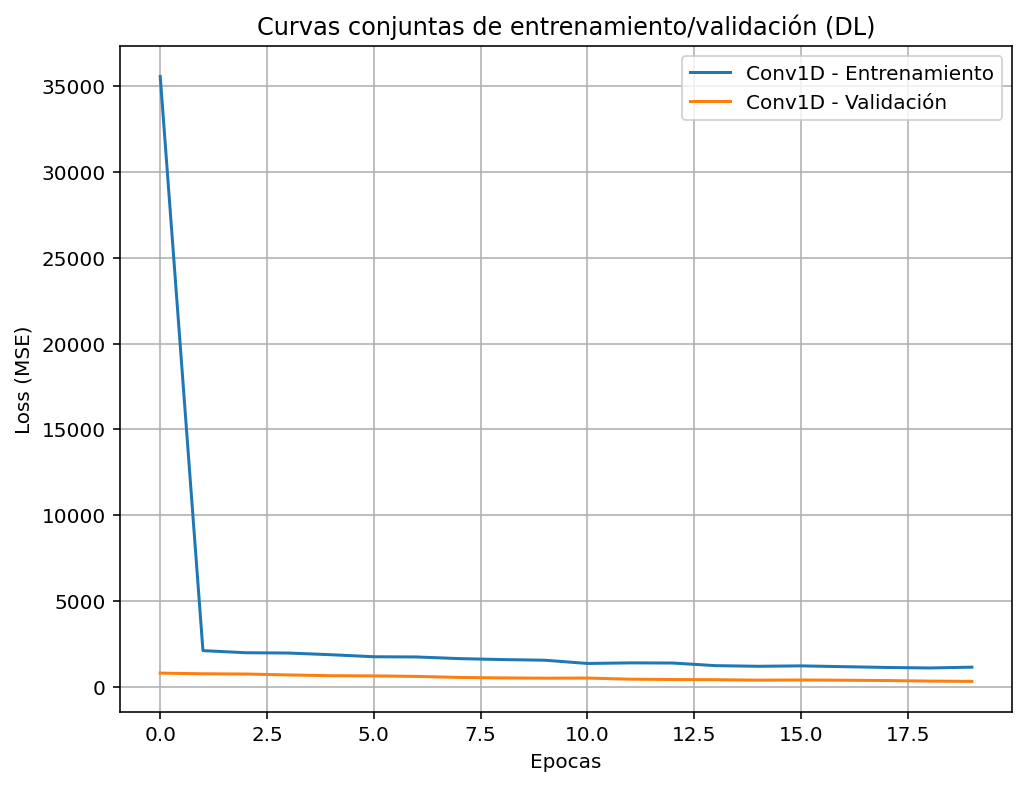
\includegraphics[width=\textwidth]{imgs/train_loss_H1.png}
        \caption{Curvas train-val loss para H=1} \label{fig:trainlossH1}
    \end{subfigure}
    \hfill
    \begin{subfigure}{0.45\textwidth}
        \centering
        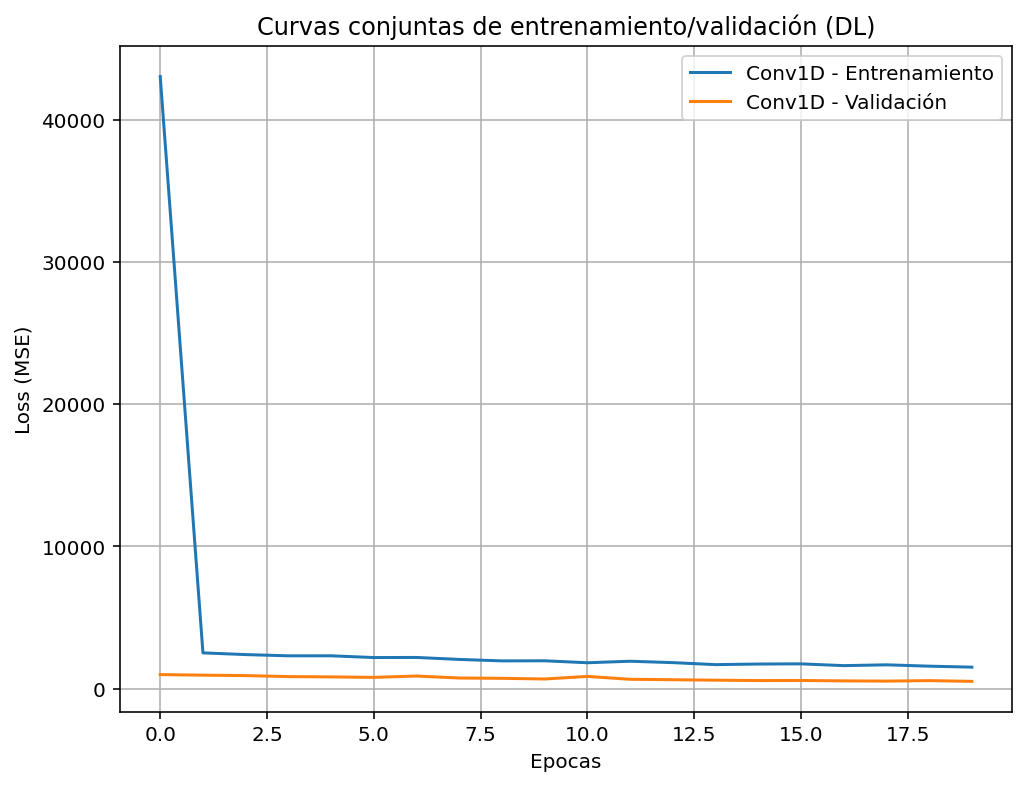
\includegraphics[width=\textwidth]{imgs/train_loss_H4.png}
        \caption{Curvas train-val loss para H=1} \label{fig:trainlossH4}
    \end{subfigure}
    \caption{Curvas train-val loss} \label{fig:trainloss}
\end{figure}

Por último, analizaremos las métricas del modelo final de bagging (cuadro \ref{cuadro:bagging}) y las compararemos con las que obtuvimos con los modelos base, tanto en la tabla \ref{cuadro:H1} como 
en la tabla \ref{cuadro:H4}. En general, vemos que para el horizonte de predicción a corto plazo mejora los modelos, mientras que en horizontes más largos tiene un rendimiento más estable.
En H=1, el $R^2$ aumentó ligeramente, desde el 0.9817 del Conv1D al 0.9882, pero con una destacable disminución de los errores, que se reducen a la mitad, pasando el RMSE de 30.50 a 16.26 
y el MAE de 11.60 a 5.57. Para H=4, el $R^2$ se mantiene prácticamente estable, ya que únicamente baja de 0.9760 a 0.9757, y los errores apenas varían, pasando el RMSE de 35.32 a 34.87 y el 
MAE de 13.31 a 13.16. De esta forma, vemos que el bagging, en general, ofrece mayor robustez y estabilidad, aportando más ventajas en horizontes cortos, y manteniéndos más estable en horizontes largos.
\begin{table}[h!]
\centering
\begin{tabular}{|c|c|c|c|c|c|c|}
\hline
\textbf{Horizonte} & \textbf{MSE} & \textbf{RMSE} & \textbf{MAE} & \textbf{R2} & \textbf{MAPE} & \textbf{EVS} \\
\hline
\textbf{H1} &  264.543  & 16.2648 &  5.5755 & 0.9882 &  6.2485 & 0.9882 \\
\hline
\textbf{H4} & 1421.3568 & 34.8701 & 13.1624 & 0.9757 & 10.8791 & 0.9757 \\
\hline
\end{tabular}
\caption{Resultados del modelo con bagging} \label{cuadro:bagging}
\end{table}

\section{Resultados} \label{resultados}
Una vez aplicadas las distintas técnicas para obtener los mejores modelos, ya tenemos decidido aquel que usaremos para realizar las predicciones. Pero, si recordamos, como explicamos 
en \ref{training}, habíamos entrenado los modelos inicialmente sobre un subconjunto de los datos, con el objetivo de agilizar las pruebas, y poder entrenar únicamente el modelo final 
con todos los datos de todas las empresas. Una vez realizadas las predicciones, se obtienen los siguientes resultados.

\begin{lstlisting}
Top 6 empresas con mayor crecimiento previsto (H=1):
CMG : Actual= 2194.45 | Pred= 2370.56 | DifAbs= 176.11 | Dif%=  8.03%
AVGO: Actual=  940.53 | Pred= 1103.11 | DifAbs= 162.58 | Dif%= 17.29%
REGN: Actual=  808.89 | Pred=  826.28 | DifAbs=  17.39 | Dif%=  2.15%
DE  : Actual=  363.31 | Pred=  378.08 | DifAbs=  14.77 | Dif%=  4.07%
MCK : Actual=  458.51 | Pred=  468.86 | DifAbs=  10.35 | Dif%=  2.26%
APD : Actual=  267.40 | Pred=  276.94 | DifAbs=   9.54 | Dif%=  3.57%
\end{lstlisting}
\begin{figure}
    \centering
    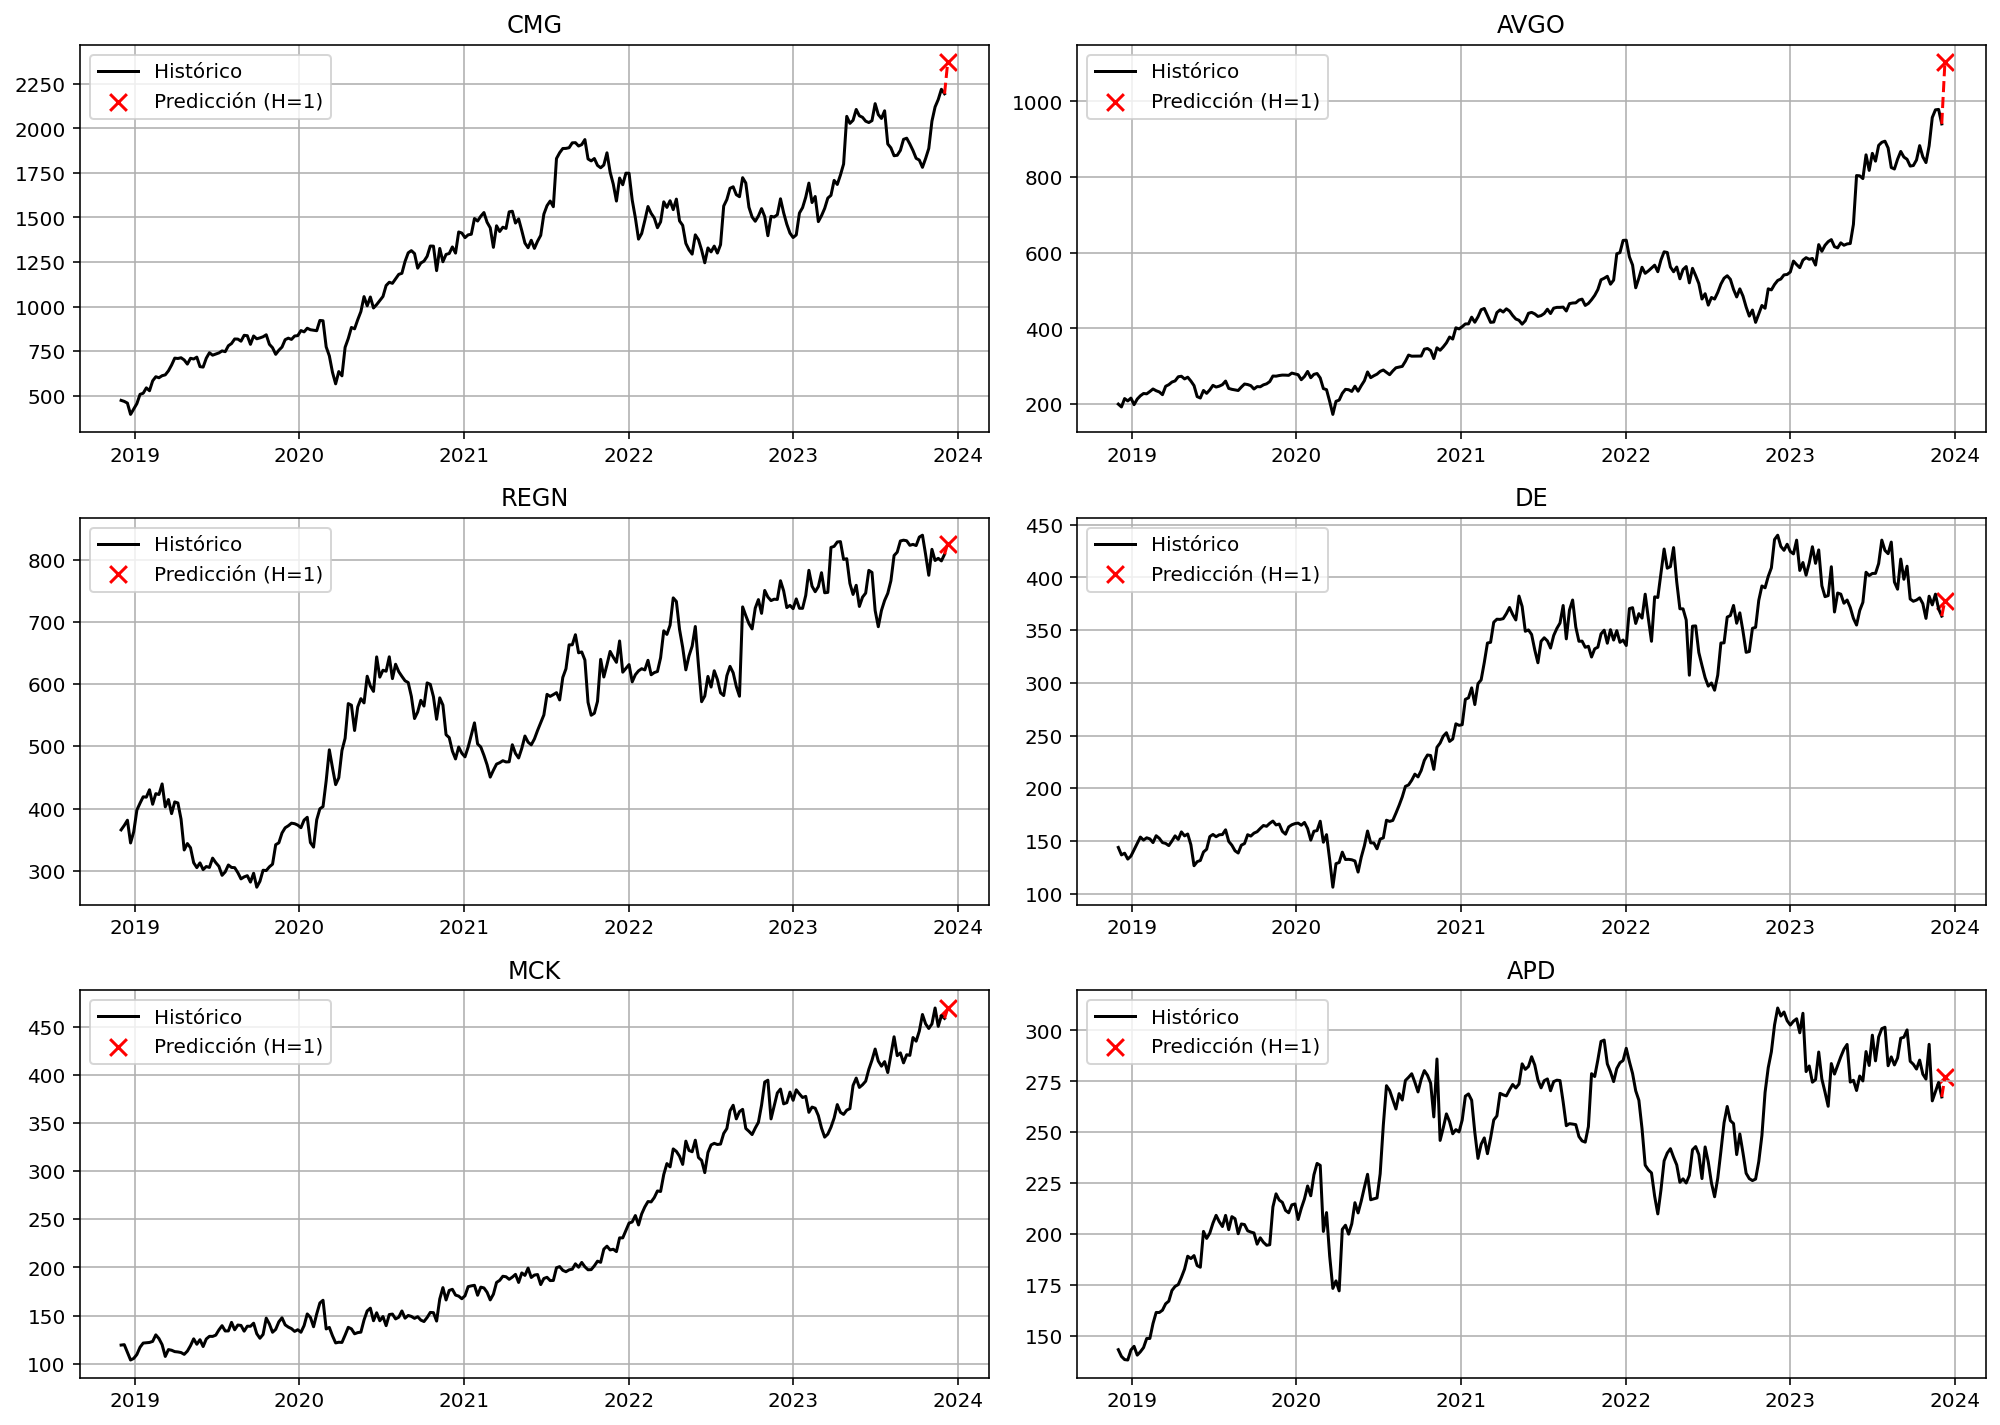
\includegraphics[width=0.6\textwidth]{imgs/grafico_H1.png}
    \caption{Predicciones para horizonte H=1} \label{fig:predsH1}
\end{figure}
En el caso de H=1, vemos que la empresa más rentable para invertir sería AVGO (Broadcom Inc.), ya que es la que proporciona una mayor crecimiento relativo, con un 17.29\% de incremento pronosticado. 
En lo que al crecimiento absoluto se refiere, la mejor empresa sería CMG (Chipotle Mexican Grill, Inc.), que nos daría un rendimiento de 176\$, pero tendríamos que invertir más dinero.
En el gráfico \ref{fig:predsH1} podemos ver estas seis empresas, graficadas su serie histórica y las predicciones en color rojo.

\begin{lstlisting}
Top 6 empresas con mayor crecimiento previsto (H=4):
Empresa: ABEV. Ultimo valor: 2.74
   +1 semana(s): Pred=4.83 | Dif=2.08 | Dif%=76.04%
   +2 semana(s): Pred=4.89 | Dif=2.14 | Dif%=78.22%
   +3 semana(s): Pred=5.03 | Dif=2.29 | Dif%=83.53%
   +4 semana(s): Pred=5.14 | Dif=2.40 | Dif%=87.47%

Empresa: MFG. Ultimo valor: 3.40
   +1 semana(s): Pred=5.12 | Dif=1.71 | Dif%=50.34%
   +2 semana(s): Pred=5.11 | Dif=1.70 | Dif%=50.00%
   +3 semana(s): Pred=5.22 | Dif=1.81 | Dif%=53.21%
   +4 semana(s): Pred=5.33 | Dif=1.92 | Dif%=56.47%

Empresa: NOK. Ultimo valor: 3.58
   +1 semana(s): Pred=5.16 | Dif=1.58 | Dif%=44.26%
   +2 semana(s): Pred=5.16 | Dif=1.58 | Dif%=44.01%
   +3 semana(s): Pred=5.27 | Dif=1.69 | Dif%=47.09%
   +4 semana(s): Pred=5.38 | Dif=1.80 | Dif%=50.28%

Empresa: TEF. Ultimo valor: 4.21
   +1 semana(s): Pred=5.37 | Dif=1.16 | Dif%=27.67%
   +2 semana(s): Pred=5.38 | Dif=1.17 | Dif%=27.72%
   +3 semana(s): Pred=5.44 | Dif=1.23 | Dif%=29.31%
   +4 semana(s): Pred=5.56 | Dif=1.35 | Dif%=32.04%

Empresa: WIT. Ultimo valor: 4.78
   +1 semana(s): Pred=5.92 | Dif=1.14 | Dif%=23.77%
   +2 semana(s): Pred=5.94 | Dif=1.16 | Dif%=24.34%
   +3 semana(s): Pred=6.00 | Dif=1.22 | Dif%=25.43%
   +4 semana(s): Pred=6.02 | Dif=1.24 | Dif%=25.92%

Empresa: NWG. Ultimo valor: 5.29
   +1 semana(s): Pred=6.36 | Dif=1.07 | Dif%=20.21%
   +2 semana(s): Pred=6.37 | Dif=1.08 | Dif%=20.34%
   +3 semana(s): Pred=6.43 | Dif=1.14 | Dif%=21.55%
   +4 semana(s): Pred=6.40 | Dif=1.11 | Dif%=21.04%
\end{lstlisting}
\begin{figure}
    \centering
    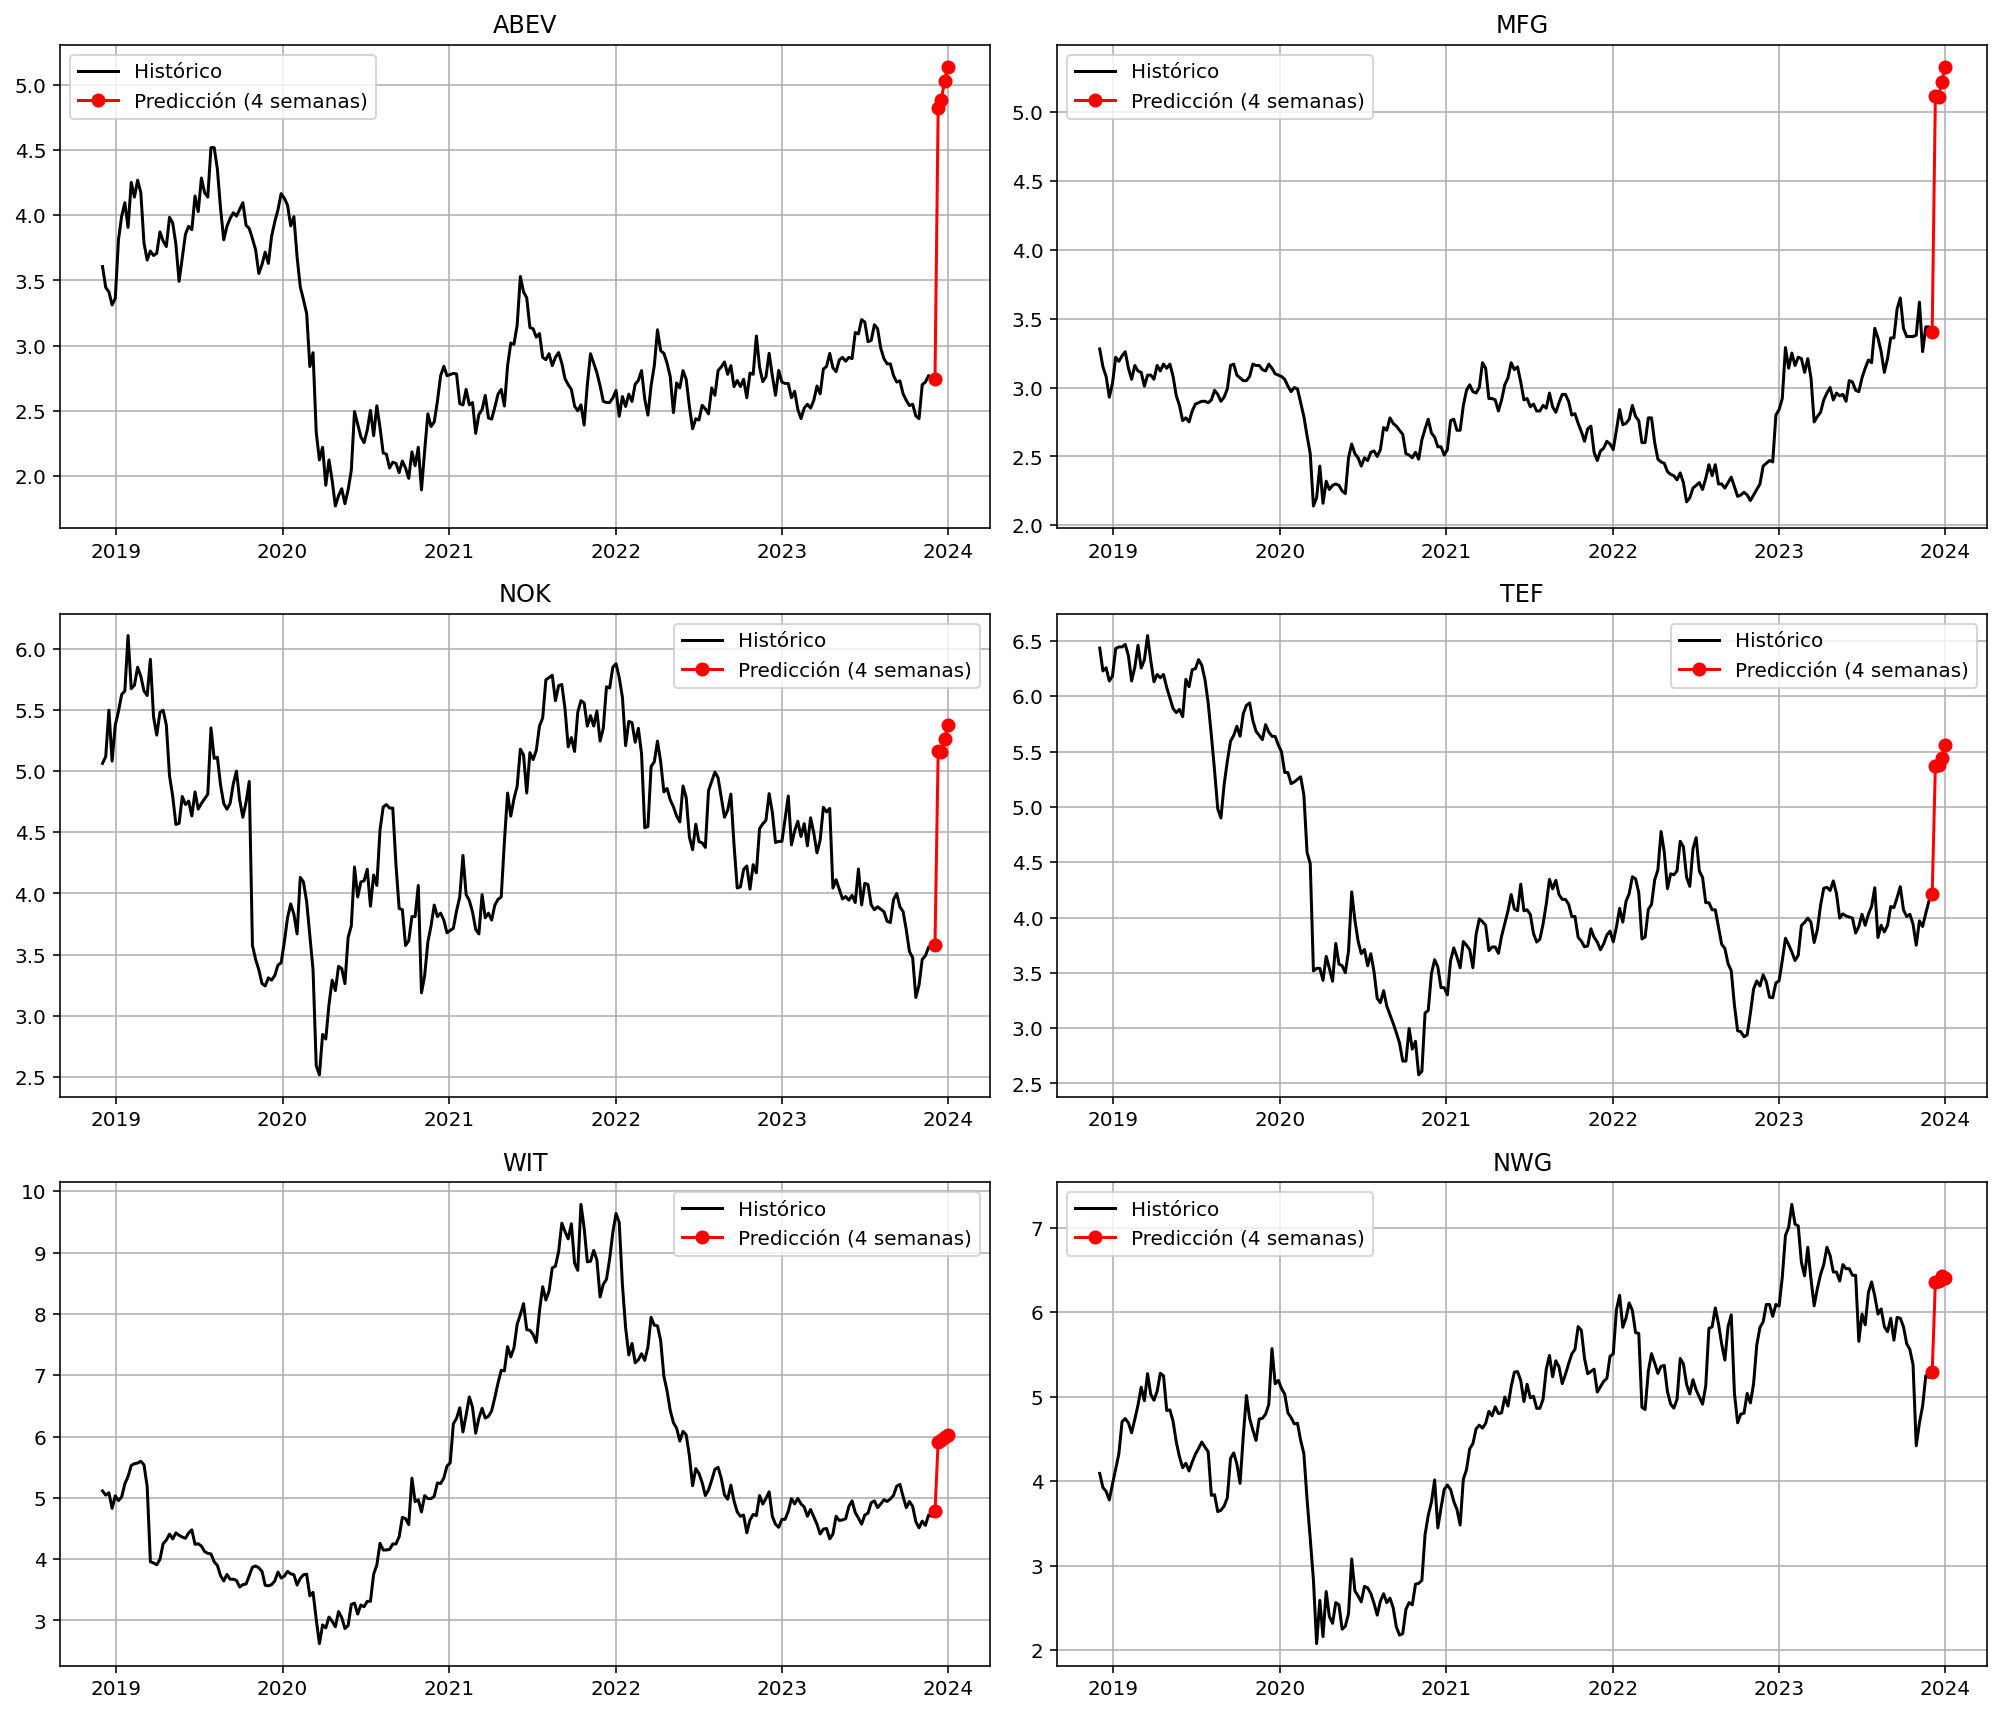
\includegraphics[width=0.6\textwidth]{imgs/grafico_H4.png}
    \caption{Predicciones para horizonte H=4} \label{fig:predsH4}
\end{figure}
En el caso de H=4, observamos que la empresa más rentable para invertir sería ABEV (Ambev S.A.), ya que es la que muestra un mayor crecimiento relativo, con un 87.47\% de incremento pronosticado.
Si atendemos al crecimiento absoluto, la mejor opción sería MFG (Mizuho Financial Group, Inc.), con un aumento proyectado de 1.92\$, aunque el importe de partida es menor que en otras compañías.
En el gráfico \ref{fig:predsH4} se representan estas seis empresas, mostrando en negro la serie histórica y en rojo las predicciones correspondientes a las cuatro semanas posteriores.
Cabe destacar, además, que las predicciones para este muestran un crecimiento inicial más abrupto, estabilizándose en las semanas posteriores, lo que indica que no es el modelo más indicado.

\begin{figure}
    \centering
    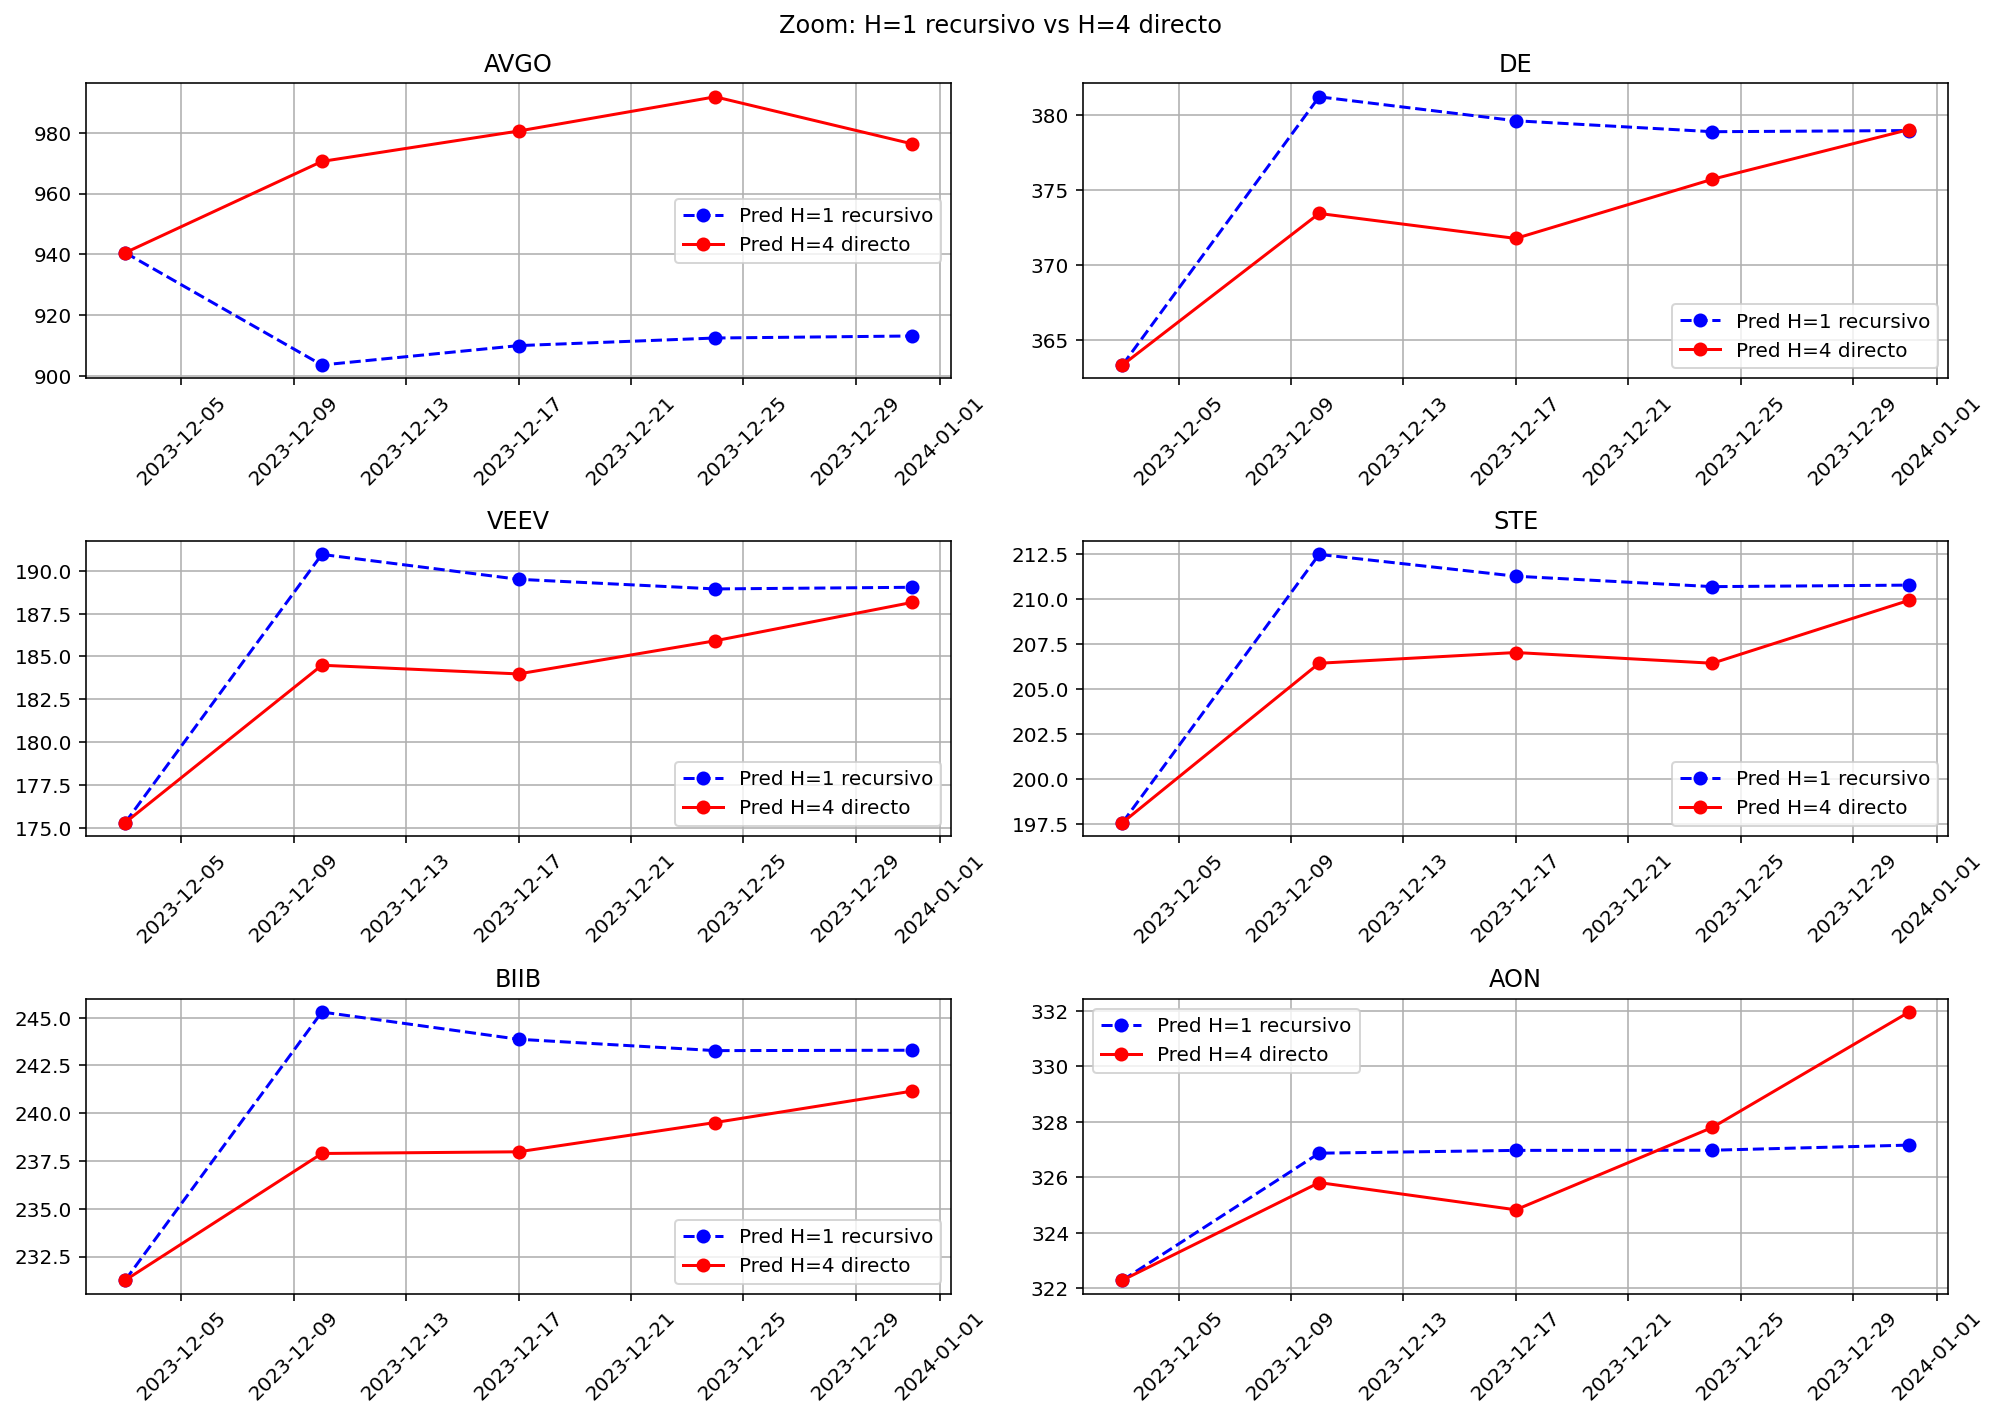
\includegraphics[width=0.6\textwidth]{imgs/grafico_comb.png}
    \caption{Comparación de predicciones para horizontes H=1 y H=4} \label{fig:combinado}
\end{figure}
Por último, analizamos el gráfico que resulta de realizar la predicción directamente con el horizonte H=4, frente a realizarla semana a semana, y retroalimentando el modelo con las nuevas predicciones. 
Podemos ver que las predicciones recursivas (en azul) tienden a capturar mejor fluctuaciones intermedias de los datos, aunque presenta más variabilidad e, indudablemente, es sensible a la acumulación
de error conforme avanza el horizonte; mientras que las predicciones directas (en rojo) generan trayectorias más suaves, aunque con un sesgo o crecimiento inicial más abrupto. Como era de esperar,
el modelo recursivo genera muy bien movimientos a corto plazo, mientras que el directo capta mejor las tendencias generales.

\section{Conclusiones} \label{conclusiones}
En este trabajo se ha desarrollado un algoritmo de Machine Learning para predecir series temporales financieras, aplicando diferentes modelos de aprendizaje automático y profundo: 
XGBoost, LightGBM, LSTM, GRU y Conv1D, con horizontes de predicción de una semana (H=1) y un mes (H=4). El objetivo del mismo era determinar en qué empresa sería más rentable invertir.

Se realizó un análisis inicial de los datos y un proceso de limpieza de los mismos, garantizando series consistentes, sin valores faltantes, y construyendo datasets supervisados con 
ventanas deslizantes. Posteriormente, se crearon y entrenaron los modelos, aplicando validación cruzada temporal para evaluar el rendimiento de los modelos evitando fugas de información.

Los resultados revelaron que el modelo convolucional ofreció las mejores métricas, logrando capturar muy bien los patrones locales de las series, seguido de los modelos basados en árboles de decisión (XGboost y LightGBM), mientras que los 
modelos de arquitecturas recurrentes (LSTM y GRU) mostraron un rendimiento inferior al esperado, probablemente por la complejidad de sus parámetros y la naturaleza de los datos.
La incorporación de la técnica de \textit{bagging} permitió incrementar, aún más, el rendimiento de los modelos, especialmente en horizontes temporales cortos.

Como ampliaciones o mejoras futuras de este trabajo, además de la puesta en producción del modelo en casos reales, el seguir ampliando los datos de entrenamiento semanalmente, conforme se vayan produciendo,
así como ampliar los datos históricos previos. También se podrían añadir a los modelos variables exógenas, como indicadores macroeconómicos o noticias financieras, para enriquecer el contexto del modelo.
También resultaría interesante poder explorar opciones más avanzadas, como transformers o redes convolucionales temporales (TCN), o probar con modelos hibridos, que combinen las fortalezas 
de las RNN y las CNN.

\renewcommand\section{\stdsection}
\section{Bibliografía} \label{bibliografia}
\begin{enumerate}
    \item Scikit-learn: \url{https://scikit-learn.org/stable/}
    \item XGBoost: \url{https://xgboost.readthedocs.io/}
    \item LightGBM: \url{https://lightgbm.readthedocs.io/}
    \item TensorFlow Keras: \url{https://keras.io/}
    \item Hyndman \& Athanasopoulos, \textit{Forecasting: Principles and Practice}: \url{https://otexts.com/fpp3/}
    \item Machine Learning Mastery, explicación del bagging: \url{https://machinelearningmastery.com/bagging-and-random-forest-ensemble-algorithms-for-machine-learning/}
    \item Validación cruzada en series temporales: \url{https://scikit-learn.org/stable/modules/cross_validation.html#time-series-split}
\end{enumerate}

\renewcommand\section{\newpage\stdsection}

\clearpage

\appendix
\section{Código EDA}\label{Anexo:EDA}
\lstinputlisting[language=Python]{EDA.py}

\section{Código para H=4}\label{Anexo:H1}
\lstinputlisting[language=Python]{code_H1.py}

\section{Código para H=1}\label{Anexo:H4}
\lstinputlisting[language=Python]{code_H4.py}

\section{Código combinado con H=1 y H=4}\label{Anexo:Comb}
\lstinputlisting[language=Python]{codigo_ML.py}
\end{sloppypar}
\end{document}
